\section{Pairwise HMM}
Pairwise Hidden Markov Model (PHMM) is probablistic generative model used for pairwise sequence alignment. Given transition and emission probability distributions, it can compute likelyhood of `similarity' as well as the most probable alignment. Furthermore, it is possible to optimize parameters by iterative procedure (EM algorithm). This one of discrete HMMs, but different from them as the length of hidden states changes dinamically according to the alighment. We will introduce PHMM using analogy to simple HMM.

\subsection{Formulation}
The main difference of PHMM from HMM comes from the uncertain alinment. We have to marginalize over all the possible alignment in order to obtain, for example, marginal likelihood. 

Let us consider the simpliest configuration of the hidden states, in which the model has three states $\mathcal{S} = \{M, X, Y\}$\footnote{$\mathcal{S} = \{\mathcal{M}, \mathcal{X}, \mathcal{Y}\}$ would be better? (notational conflict)}, Match state $M$, X insertion state $X$, and $Y$ insertion state (Fig.\ref{fig:hidden_states}). 

Let $\mathcal{D}= \{\vec{x}, \vec{y} \}$ be observed data, each of which contains $N$ sequences $\vec{x} = (\vec{x}^1, ..., \vec{x}^N)$, $\vec{y} = (\vec{y}^1, ..., \vec{y}^N)$. The $n$-th sequences are $\vec{x}^n = (x^n_1, ..., x^n_{T^n_{x}})$ and $\vec{y}^n = (y^n_1, ..., y^n_{T_{yn}} )$ where $T_{x}^n$ and $T_{y}^n$ are the length of the $\vec{x}^n$ and $\vec{y}^n$, respectively. 
%Unlike the normal HMM, we here introduce 2d-grid hidden states (Fig.\ref{fig:hidden_states_2d}) to keep the notation simple. Let $\vec{w} = (\vec{w}^1, ...,\vec{w}^N)$ be hidden states. 
%$\vec{w}^n$ is 2d-grid hidden variables of size $T^n_{x} \times T^n_{y}$. 
%The $w_{t, u}$ represents the hidden state corresponding to the output $(x_t, y_u)$. This formulation enable us to express all the possible alignment, which corresponds to the all the possible paths from $w_{1,1}$ to $w_{T_x, T_y}$. 
The joint distribution of the observed and the hidden variables are given by
\begin{eqnarray}
%  p(X, Y, W) = p(W_{1,1}) \prod_{(t_i, u_i)\rightarrow(t_j, u_j) \in \mathcal{P}} p(W_{t_j, u_j}|W_{t_i, u_i}) \
%p(\vec{X}, \vec{Y}, \vec{W}) = p(W_{1,1}) \prod_{t=2}^{T_X} \prod_{u=2}^{T_Y} p(W_{t, u}|pa(W_{t, u})) \prod_{t=1}^{T_X} \prod_{u=1}^{T_Y} p(X_t, Y_u | W_{t,u})
p(\vec{X}, \vec{Y}, \vec{Z}) = p(Z_{1}) \prod_{t=2}^{T} p(Z_t|Z_{t-1}) \prod_{t=1}^{T} p(X_{t_x(t)}, Y_{t_y(t)} | Z_t)
\end{eqnarray}
where $t_x(t)$ and $t_y(t)$ are determined by hidden states sequence $\vec{Z}$.
\begin{eqnarray}
  t_x(t) &=& 1 + \sum_{i=1}^{t-1} I(Z_i \in \{M, X\}) \\
  t_y(t) &=& 1 + \sum_{i=1}^{t-1} I(Z_i \in \{M, Y\})
\end{eqnarray}
where $I(\cdot)$ is indicator function.

\begin{figure}
  \centering
  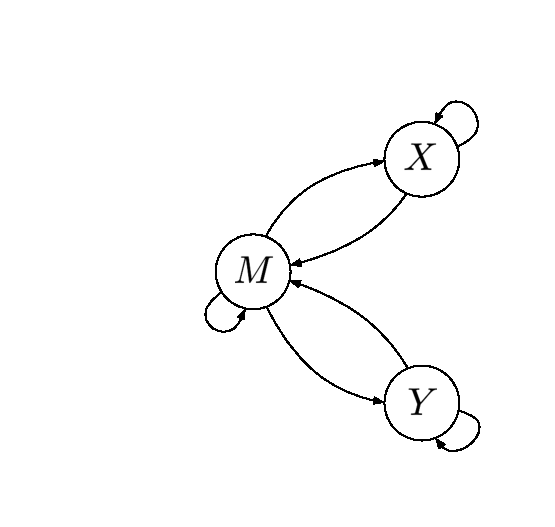
\includegraphics[width=.6\linewidth]{hidden_states.pdf}
  \caption{{\bf The simpliest configuration of hidden states}}
  \label{fig:hidden_states}
\end{figure}

% \begin{figure}
%   \centering
%   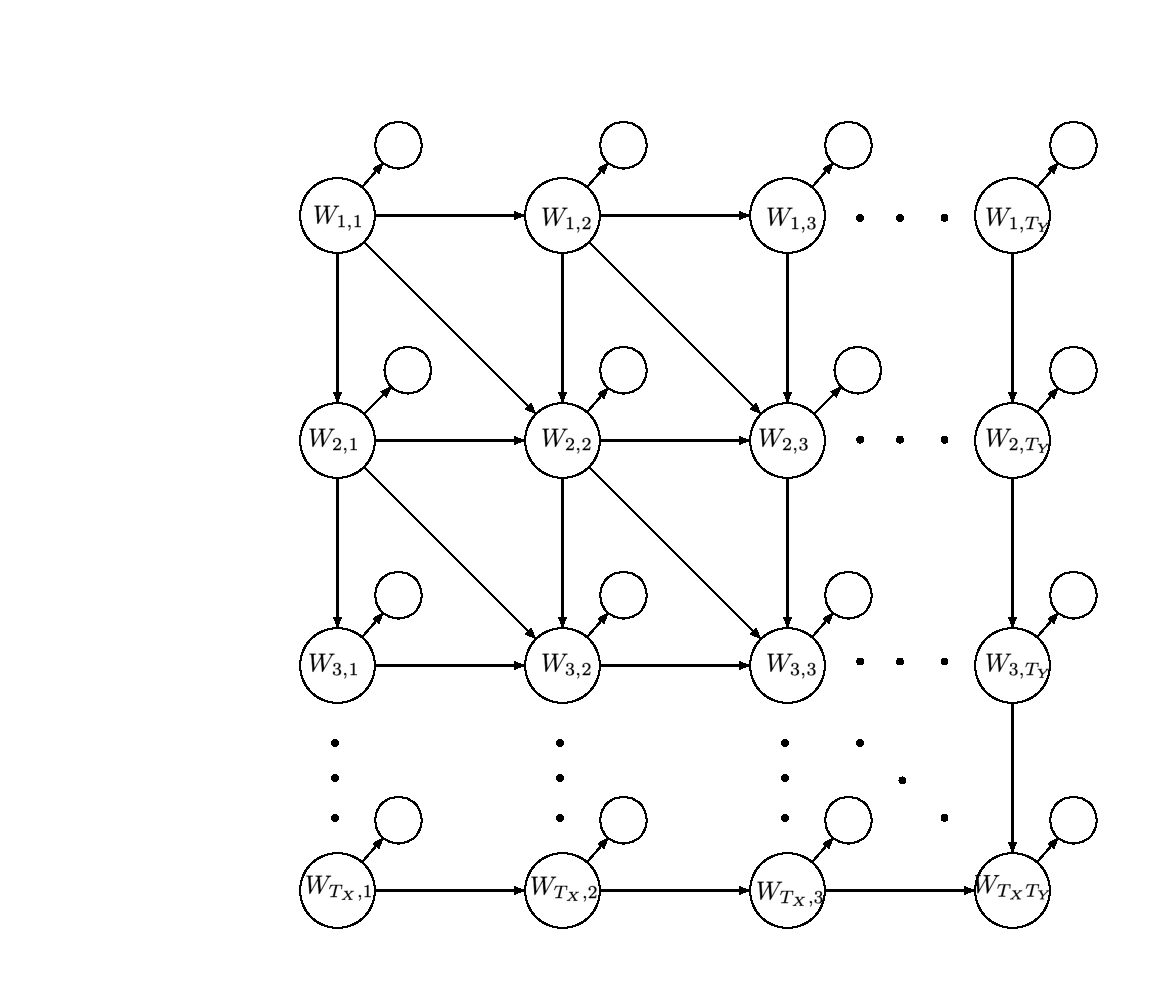
\includegraphics[width=1\linewidth]{hidden_states_2d.pdf}
%   \caption{{\bf 2-D grid hidden states}}
%   \label{fig:hidden_states_2d}
% \end{figure}

\subsection{Forward-Backward Algorithm}
We introduce PHMM version of Forward-Backward Algorithm. 
It is similar to that of the ordinary HMM, but a bit different because of the uncertain alignment. 
We need to give the formulation for each hidden states because the procedure of DP is a bit different each other.
We start with the case where the target hidden variable is $M$ state. 
Define the smoothed marginal $p(z_{t, u} = M | \vec{x}, \vec{y})$ where $z_{t, u}$ is the hidden variable that corresponds to $t, u$ (how can I explain this???). Note that we cannot compute scaling version so forward and backward algorithm are slightly modified so that it does not contain scaling.
\begin{eqnarray}
  p(z_{t,u} = M | \vec{x}, \vec{y}) 
                            &=& \frac{ p(z_{t, u}=M , \vec{x}_{1:t}, \vec{y}_{1:u}) p(\vec{x}_{t+1:T_x}, \vec{y}_{u+1:T_y} | z_{t, u}= M) } {p(\vec{x}_{1:T_x}, \vec{y}_{1:T_y})} \nonumber \\
                            &=& \frac{1}{c_{t,u}} f_{M, t, u} b_{M, t, u}
\end{eqnarray}
Forward variable $f_{M, t, u}$, backward variable $b_{M, t, u}$ and normalization constant $c_{t, u}$ are difined as:
\begin{eqnarray}
  f_{M, t, u} &=& p(z_{t, u}=M | \vec{x}_{1:t}, \vec{y}_{1:u}) \\
  b_{M, t, u} &=& p(\vec{x}_{t+1:T_x}, \vec{y}_{u+1:T_y} | z_{t, u}= M) \\
  c_{t, u}    &=& p(\vec{x}_{t+1:T_x}, \vec{y}_{u+1:T_y}| \vec{x}_{1:t}, \vec{y}_{1:u})
\end{eqnarray}
Similarly, the smoothed marginal of the hidden state $X$ and $Y$ are written as:
\begin{eqnarray}
p(z_{t,u} = X | \vec{x}, \vec{y}) &=& \frac{ p(z_{t, u}=X, \vec{x}_{t+1:T_x}, \vec{y}_{u:T_y}| \vec{x}_{1:t}, \vec{y}_{1:u-1}) } {p(\vec{x}_{t+1:T_x}, \vec{y}_{u:T_y}| \vec{x}_{1:t}, \vec{y}_{1:u-1})} \nonumber\\
                            &=& \frac{ p(z_{t, u}=X | \vec{x}_{1:t}, \vec{y}_{1:u-1}) p(\vec{x}_{t+1:T_x}, \vec{y}_{u:T_y} | z_{t, u}= X) } {p(\vec{x}_{t+1:T_x}, \vec{y}_{u:T_y}| \vec{x}_{1:t}, \vec{y}_{1:u-1})} \nonumber \\
                            &=& \frac{1}{c_{t,u-1}} f_{X, t, u} b_{X, t, u} \\
p(z_{t,u} = Y | \vec{x}, \vec{y}) &=& \frac{ p(z_{t, u}=Y, \vec{x}_{t:T_x}, \vec{y}_{u+1:T_y}| \vec{x}_{1:t-1}, \vec{y}_{1:u}) } {p(\vec{x}_{t:T_x}, \vec{y}_{u+1:T_y}| \vec{x}_{1:t-1}, \vec{y}_{1:u})} \nonumber\\
                            &=& \frac{ p(z_{t, u}=Y | \vec{x}_{1:t-1}, \vec{y}_{1:u}) p(\vec{x}_{t:T_x}, \vec{y}_{u+1:T_y} | z_{t, u}= Y) } {p(\vec{x}_{t:T_x}, \vec{y}_{u+1:T_y}| \vec{x}_{1:t-1}, \vec{y}_{1:u})} \nonumber \\
                            &=& \frac{1}{c_{t-1,u}} f_{Y, t, u} b_{Y, t, u}
\end{eqnarray}
where forward and backward variables are defined as:
\begin{eqnarray}
  f_{X, t, u} &=& p(z_{t, u}=X | \vec{x}_{1:t}, \vec{y}_{1:u-1}) \\
  b_{X, t, u} &=& p(\vec{x}_{t+1:T_x}, \vec{y}_{u:T_y} | z_{t, u}= X)  \\
  f_{Y, t, u} &=& p(z_{t, u}=Y | \vec{x}_{1:t-1}, \vec{y}_{1:u}) \\
  b_{Y, t, u} &=& p(\vec{x}_{t:T_x}, \vec{y}_{u+1:T_y} | z_{t, u}= Y) 
\end{eqnarray}
Now we can construct the procedure of DP. Let us write down the recurrence relation in the case where $z_{t,u} = M$. (it is hard to compute the denomitor so we should give up scaling? ... denomiter differ according to the hidden states)
\begin{eqnarray}
f_{M, t, u} &=& p(z_{t, u}=M | \vec{x}_{1:t}, \vec{y}_{1:u}) \nonumber \\
            &=& \frac{p(z_{t, u}=M, x_t, y_u | \vec{x}_{1:t-1}, \vec{y}_{1:u-1})} {p(x_t, y_u | \vec{x}_{1:t-1}, \vec{y}_{1:u-1})} \nonumber \\
            &=& \frac{p(x_t, y_u |z_{t, u}=M) p(z_{t, u}=M| \vec{x}_{1:t-1}, \vec{y}_{1:u-1})} {p(x_t, y_u | \vec{x}_{1:t-1}, \vec{y}_{1:u-1})} \nonumber\\
            &=& \frac{p(x_t, y_u |z_{t, u}=M) p(z_{t, u}=M| \vec{x}_{1:t-1}, \vec{y}_{1:u-1})} {p(x_t, y_u | \vec{x}_{1:t-1}, \vec{y}_{1:u-1})} \nonumber\\
            &=& \frac{p(x_t, y_u |z_{t, u}=M)} {p(x_t, y_u | \vec{x}_{1:t-1}, \vec{y}_{1:u-1})} \times \nonumber \\
&&\big[p(z_{t, u}=M| z_{t-1, u-1} = M)p(z_{t-1,u-1} = M | \vec{x}_{1:t-1}, \vec{y}_{1:u-1}) + \nonumber \\
&&\ p(z_{t, u}=M| z_{t-1, u} = X)p(z_{t-1,u} = X | \vec{x}_{1:t-1}, \vec{y}_{1:u-1}) + \nonumber \\
&&\ p(z_{t, u}=M| z_{t, u-1} = Y)p(z_{t,u-1} = Y | \vec{x}_{1:t-1}, \vec{y}_{1:u-1})  \big]\nonumber \\
&=& \frac{\psi_{M, t, u}}{d_{t,u}} [\beta_{M,M} f_{M,t-1,u-1} + \beta_{X,M} f_{t-1, u} + \beta_{Y,M} f_{Y, t, u-1}]\\
  b_{M, t, u}
            &=& p(\vec{x}_{t+1:T_x}, \vec{y}_{u+1:T_y} | z_{t, u}= M) \nonumber \\
            &=& \sum_{k \in \mathcal{S}}p(\vec{x}_{t+1:T_x}, \vec{y}_{u+1:T_y} z_{t+1, u+1} = k| z_{t, u}= M) \nonumber\\
            &=& \sum_{k \in \mathcal{S}}p(\vec{x}_{t+1:T_x}, \vec{y}_{u+1:T_y}|z_{t+1, u+1}=k) p(z_{t+1, u+1} = k| z_{t, u}= M)\nonumber \\ 
            &=& p(x_{t+1}, y_{u+1}|z_{t+1, u+1}=M)p(\vec{x}_{t+2:T_x}, \vec{y}_{u+2:T_y}|z_{t+1, u+1}=M) p(z_{t+1, u+1} = M| z_{t, u}= M) +\nonumber \\ 
            && p(x_{t+1}|z_{t+1, u+1}=X)p(\vec{x}_{t+2:T_x}, \vec{y}_{u+1:T_y}|z_{t+1, u+1}=X) p(z_{t+1, u+1} = X| z_{t, u}= M) + \nonumber \\ 
            && p(y_{t+1}|z_{t+1, u+1}=Y)p(\vec{x}_{t+1:T_x}, \vec{y}_{u+2:T_y}|z_{t+1, u+1}=Y) p(z_{t+1, u+1} = Y| z_{t, u}= M) \nonumber \\ 
            &=& \psi_{M, t+1, u+1} b_{M, t+1, u+1} \beta_{M,M} + \psi_{X, t+1, u} b_{X, t+1, u} \beta_{M,X} + \psi_{Y, t, u+1} b_{Y, t, u+1} \beta_{M,Y}
\end{eqnarray}
where $d_{t,u}$ is defined as:
\begin{eqnarray}
  d_{t,u} = {p(x_t, y_u | \vec{x}_{1:t-1}, \vec{y}_{1:u-1})} 
\end{eqnarray}
(MEMO: forward... from index is different, output index is the same. backward... to index is the same, output index is different)The recurrence relation could be obtain in the same way for the hidden state $X$ and $Y$. Before showing them, let us introduce some supporting variables to make the notation simpler. Define $\delta_{x,k}$ and $\delta_{y,k}$ as:
% \begin{eqnarray}
%        \frac{p(x_t, y_u |z_{t, u}=M) \sum_{k \in \mathcal{S}}p(z_{t, u} |z_{t - \delta_{x,k}, u-\delta_{y,k}}=k)
% p(z_{t - \delta_{x,k}, u-\delta_{y,k}}=k | \vec{x}_{1:t-\delta_{x,k}}, \vec{y}_{1:u-\delta_{y,k}}) }{p(x_t, y_u | \vec{x}_{1:t-1}, \vec{y}_{1:u-1}) }
% \end{eqnarray}
\begin{eqnarray}
(\delta_{x, k}, \delta_{y, k}) =  
  \begin{cases}
    (1,1) \quad \mbox{if} \quad k = M \\
    (1,0) \quad \mbox{if} \quad k = X \\
    (0,1) \quad \mbox{if} \quad k = Y
  \end{cases}
\end{eqnarray}



\subsection{EM}


